\chapter{Electric Fields}

\section{Introduction}

One of the fundamental concepts used to describe electric phenomena is that of the electric field. We explore the field concept experimentally by measuring lines of equal electric potential on carbon paper and then constructing the electric field lines that connect them.

\section{Theory}

\subsection{Fields}

A \underline{field} is a function in which a numerical value associated with a physical quantity is assigned to every point in space. For example, each point in the United States may be assigned a temperature (that we measure with a thermometer at that position), as shown in figure \ref{fig:temp_field}. Thus, temperature as a function of location is called the ``temperature field''. The temperature field is an example of a scalar field, since the value assigned to each location is a scalar.

\begin{figure}[h]
    \begin{center}
        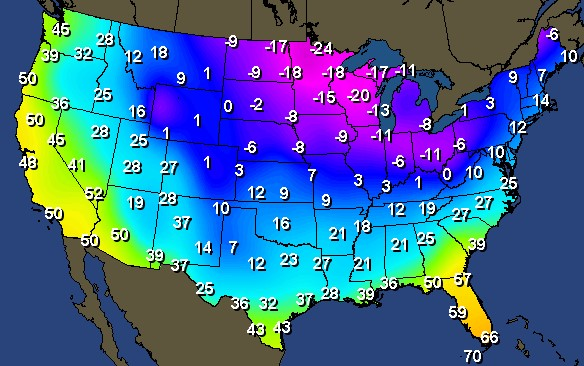
\includegraphics[width=0.5\textwidth]{./Exp1/pic/tempfield.jpg}
    \end{center}
    \caption{Temperature of Different Places in the United States}
    \label{fig:temp_field}
\end{figure}

The electric field (as well as the magnetic field) is a vector field, because a vector (rather than a scalar) is associated with each position. The direction and magnitude of an electric field at any point in space tells you the direction and magnitude of electric force that a  unit test charge would experience at this position. \myskip

A line that is formed by connecting electric field vectors and follows the direction of the field is called a \underline{field line}. A field is considered uniform if the field lines are parallel. The potential associated with such a field increases linearly with the distance traveled along the field lines.

\subsection{Equipotential Contours for Gravity}

A topographical map is a map with lines that indicate contours of the same height. On such a map, a mountain may look like figure \ref{fig:topograph}

\begin{figure}[h]
    \begin{center}
        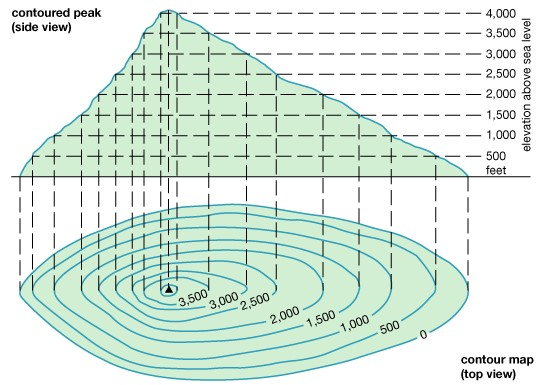
\includegraphics[width=0.4\textwidth]{./Exp1/pic/contourmap.jpg}
    \end{center}
    \caption{A Topographical Map}
    \label{fig:topograph}
\end{figure}

These contours of the same height $(h)$ are equi-height lines or, if you think in terms of potential energy $(U = mgh)$, they are equipotential lines. That is, every point on the contour has the same value of potential energy. So as you move along a contour, you do not change height, and therefore you neither gain nor lose potential energy. Only as you step up or down the hill do you change the energy. \myskip

There are a few general properties of equipotential contours:
\begin{itemize}
    \item They never intersect. (A single point cannot be at two different heights at the same time, and
therefore it cannot be on two different contours.)
    \item They close on themselves. (A line corresponding to constant height cannot just end.)
    \item They are smooth curves, as long as the topography has no sharp discontinuities (like a cliff).
\end{itemize}

\subsection{Analogy between Electric and Gravitational Potentials}

Electric potential is analogous to gravitational potential energy. Of course, gravitational potential energy arises from any object (with mass), whereas the electric potential arises only from charged objects. \myskip

As in mechanics, the absolute value of potential is not important. The differences in potential are the quantities that have physical meaning. In a real problem, it is usually best to choose a reference point, define it as having zero potential, and refer to potentials at all other points relative to the that point. Similarly, topographic height is usually reported relative to the reference at sea level.

\subsection{Field Lines}

Let's exploit our analogy of mountains and valleys a bit further for electric fields. Electric field lines indicate the electric force on a test charge (magnitude and direction). Gravitational field lines tell us about the gravitational force on a test mass (magnitude and direction) -- the direction it tends to roll down the hill and the acceleration it experiences during its journey. So if we carefully track a marble as we roll it down the hill in small increments, we can obtain a ``field-line''.  \myskip

What is the characteristic of a field line? Think about placing a marble on an inclined hillside.  Which way will it roll if you release it? It will always roll in the direction of steepest descent, and this direction is always perpendicular to the contours that indicate equal height (which we have been referring to as equipotential lines). \myskip

So it is for the electric case: if we know the equipotential lines, we can draw the field lines such that each one is perpendicular to each equipotential line. Figure \ref{fig:equi_field} and \ref{fig:field_dipole} both show equipotential lines (dashed lines) and the corresponding field lines (solid lines).

\begin{figure}[h]
    \begin{center}
        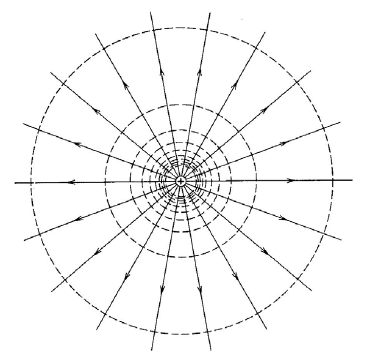
\includegraphics[width=0.5\textwidth]{./Exp1/pic/image3.png}
    \end{center}
    \caption{Equipotential Lines and Field Lines of a Single Charge}
    \label{fig:equi_field}
\end{figure}

Keep in mind that when equipotential lines are closer together, the potential is changing faster! This means we have steeper changes in height for gravitational field lines for example.

\begin{figure}[h]
    \begin{center}
        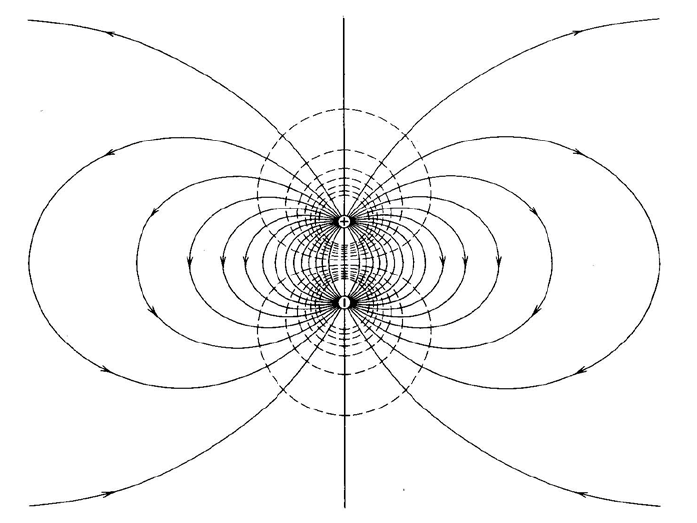
\includegraphics[width=0.6\textwidth]{./Exp1/pic/image4.png}
    \end{center}
    \caption{Equipotential Lines and Field Lines of a Pair of Opposite Charges}
    \label{fig:field_dipole}
\end{figure}

There are also a few rules for field lines:
\begin{itemize}
    \item Field lines always begin and end on charges. (They often terminate on material surfaces, but that is because there are charges on those surfaces.)
    \item They never intersect each other (except at electric charges, where they also terminate).
    \item They always intersect equipotential lines perpendicularly!
    \item They are usually smoothly continuous (except if they terminate).
\end{itemize}

\subsection{Metal Surfaces}

It turns out that for electrical phenomena, metals are equipotentials. So, by using metals, we can impose some unusually shaped equipotential lines and determine the corresponding field lines. \myskip

Metals are always equipotentials because:
\begin{enumerate}
    \item they are excellent conductors of electric charge, and
    \item they have an abundant supply of freely moving negative charges (electrons).
\end{enumerate}

Based on these two properties, we can understand that, if a field line were to penetrate a metal surface, these electrons would feel electric forces to move them through the material in the direction opposite to that of the electric field (since they are negative) until they would be forced to stop upon encountering the metal surface on the other side. Therefore, the free electrons ultimately distribute themselves along the surface of the metal so that there is a net negative charge on one side of the conductor and a net positive charge on the other (from where the electrons have fled). This realignment of the free electrons creates a field that precisely cancels the imposed field resulting in no net field, and the \underline{remaining} free charges inside the conductor then feel no force and don't move! Hence, field lines imposed from outside always end on metal surfaces (which they intersect perpendicularly), and the surface (with the entire interior) is an equipotential.

\subsection{Electric Shielding Theorem}

As just discussed, whenever a piece of metal is placed in an electric field, the entire metal will remain an equipotential. That is, every point in the metal will be at the same potential as every other point. No field lines penetrate through metals. \myskip

What happens if we take an enclosed container of metal of arbitrary shape, say a tin can, and put it into an electric field? Since no field gets through the metal, there must be no electric field inside the can. This means that every point inside the container, as well as all points on the container surface must be at the same potential. (If they were not, then there would be differences in the potential and therefore an electric field.) \myskip

Let's return to our analogy of gravity equipotentials in hills and valleys, with field lines in the direction a marble would roll down the hill. Consider how a frozen lake would look on such a contour map. The surface of the lake has the same gravitational potential energy at all points, therefore if you place a marble on the frozen surface of the lake, the marble will not roll anywhere. In other words, there is no component of the gravitational field along the surface of the lake to push the marble. Similarly, there is no electric field on the inside of a closed metal container to push the charges around, and the entire interior is therefore a constant equipotential surface.

\subsection{Remarks for Experts}

\begin{enumerate}
    \item The gravitational analogy operates in only two dimensions: the horizontal coordinates describing the surface of the lake. When discussing electrical fields we should, in principle, take into account all three dimensions. The analogy of the lake surface for the electrical case is the entire volume (three dimensions) of the interior of the can. For this experiment, we ``cheat'' a little by looking at electric field within a two dimensional world of slightly conducting paper. But the field and potential arrangements are as one expects for electrostatic phenomena in a two dimensional system.
    \item To shield electric field, we actually don't need a metallic surface that is completely closed; a closed cage of wire mesh (Faraday cage) is sufficient. So a sedan will work like a Faraday cage, but a convertible will not since it is not closed at the top.
\end{enumerate}

\section{Experiments}

In this experiment, we use metals on slightly conductive paper, probes and alligator clips  to determine different equipotential and field configurations. Each metal shape (point sources, parallel plates, and conducting loop) on the conductive paper is an equipotential curve. You will make observations on the conductive paper then draw equipotentials and electric field lines of different equipotential shapes on the white grid papers. Do NOT write anything on the conductive paper. See figure \ref{fig:equip_setup}   
\begin{figure}[h]
    \begin{center}
        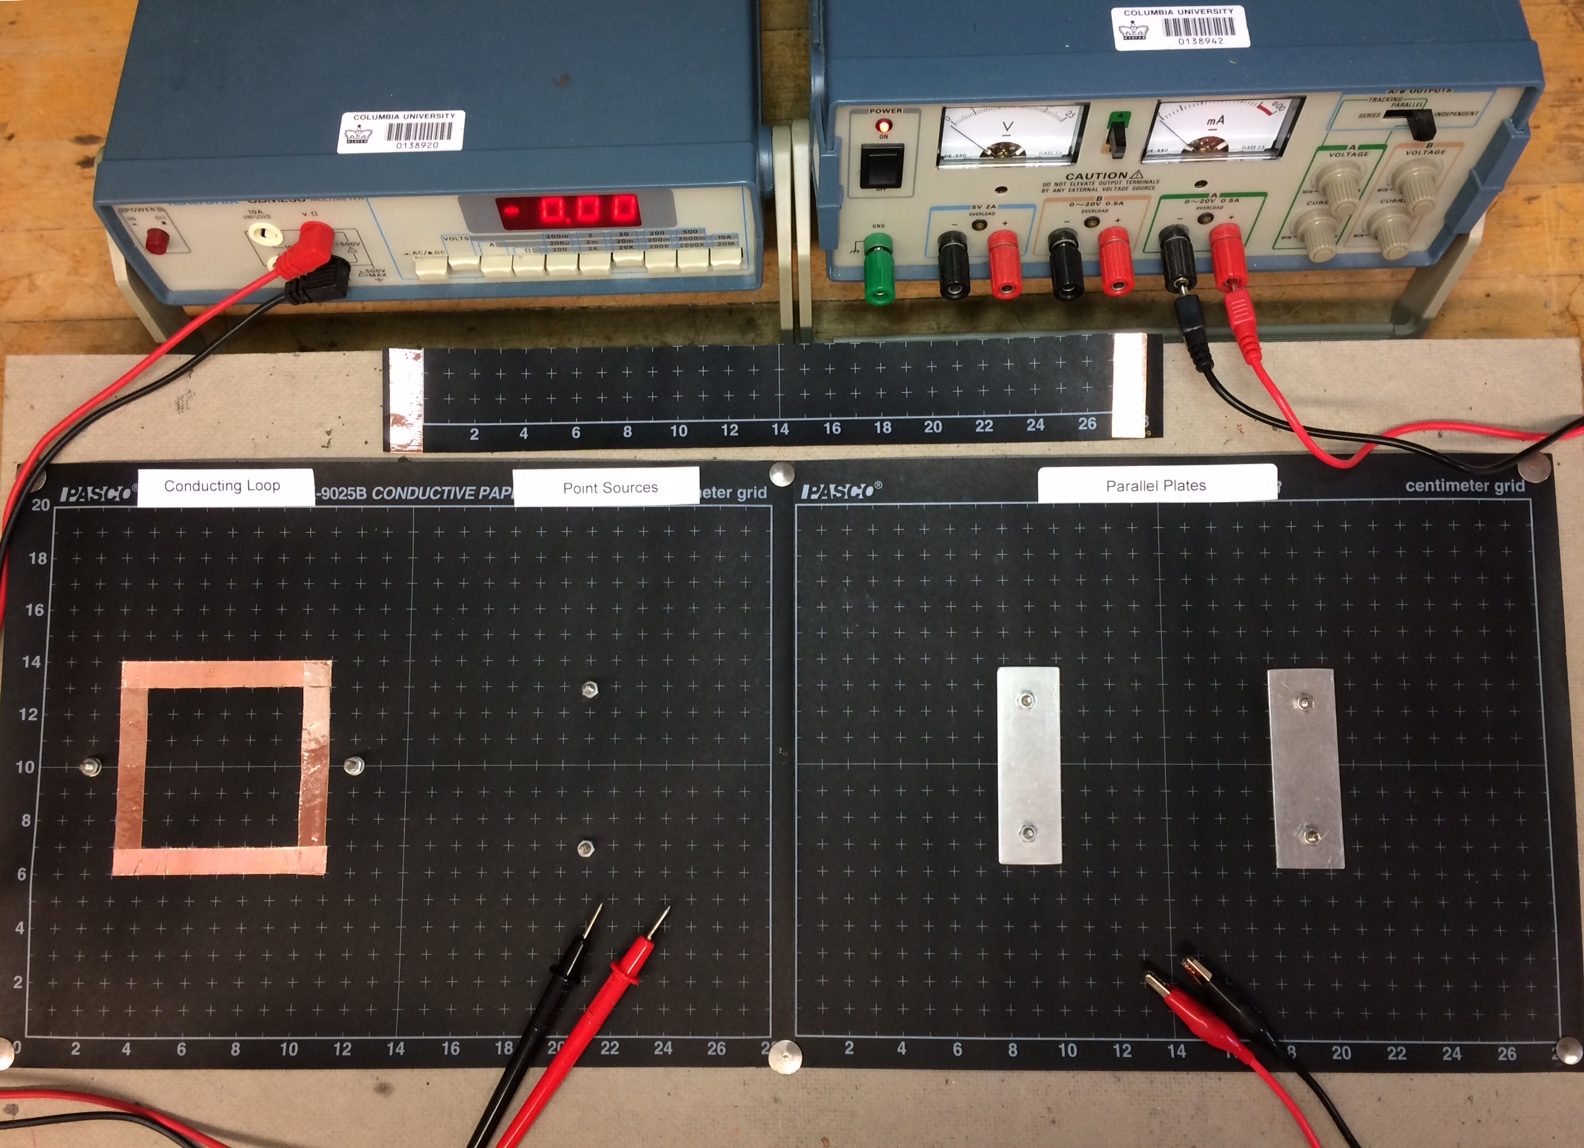
\includegraphics[width=0.6\textwidth]{./Exp1/pic/Picture1.png}
    \end{center}
    \caption{Equipment setup}
    \label{fig:equip_setup}
\end{figure}

\myskip
\noindent Hints:

    \begin{enumerate}
        \item You get the best results if you stay at least 1-2cm away from the edges of the paper. Also, make sure that the probes are always in contact with the paper. (Otherwise the experiment does not work!) Be careful not to make holes on the conductive paper.
        \item Make sure you are not accidentally touching the paper when making measurements!
    \end{enumerate}

\subsection{Setup of the Voltage Source}

\begin{enumerate}
    \item ``OUTPUT A'' of the power supply will be used in this experiment to provide a constant potential difference of 10 volts.
    \item Turn the ``A VOLTAGE'', the ``A CURRENT'', the ``B VOLTAGE'', and the ``B CURRENT'' control knobs located on the right side of the front panel counterclockwise to the ``MIN'' position.
    \item Set the ``A/B OUTPUT'' switch located on the upper right of the front panel to the ``INDEPENDENT'' setting, and set the ``A/B METER'' switch located between the two meters on the front panel to the ``A'' setting.
    \item Turn the power on by using the button located on the left of the front panel.
    \item Slowly turn the ``A VOLTAGE'' output knob until the voltage reads 10 volts. After doing this, do not make any further changes on the power supply for the remainder of the experiment. (The current meter will stay at a zero reading.)
    \item Connect the banana plugs of the alligator cables to the ``A OUTPUT ($0\sim 20\,\mathrm{V}\  0.5\,\mathrm{A}$)'' of the power supply (red and black poles).
\end{enumerate}

NOTE: To use the digital multimeter as an appropriate voltmeter for this experiment: turn the multimeter power on, select ``DC'' (button in out position), select ``VOLTS'' (push button in), set range to ``2 VOLTS'', and connect your voltage-measuring probes to the ``$\mathrm{V}$--$\Omega$'' and the ``COM'' jacks.

\subsection{Equipotential and Field Lines}

\begin{enumerate}
    \item Connect two banana plugs to the output of the power supply (black and red poles) as described in the last step of the previous part. The alligator clips are your output pins.
    \item Take the black probe and connect one end to the black pole of the multimeter. This will be your reference probe. Take the red probe and plug it into the red pole of the multimeter. This will be your measuring probe.
    \item Connect the alligator clips to the point sources on the conductive paper to create two point sources with opposite charges.
    \item Place the reference probe at an arbitrary position between the two point sources and move the measuring probe until the multimeter shows a value of zero. This means that the two points are at the same potential. Mark this position with one of the red markers on the white grid paper provided. Search for more equipotential points until you have enough to draw an equipotential contour connecting them. Do not to push the probe hard on the conductive paper to avoid making a hole on it. 
    \item Move the reference probe to a new position and construct another equipotential line on the white grid paper.
    \item Repeat for a total of about 5 equipotential lines.
    \item Given these equipotential lines, draw about 5 field lines on the white paper grid using the yellow pen. Remember that the field lines and equipotential lines always intersect perpendicularly.
    \item Do your equipotential and field lines show the symmetries you would expect for this system? Just what symmetries does/should this system have?
    \item Obtain the equipotential and field lines for the parallel-plate configuration as well. Clip one alligator at a screw on each plate to produce a potential difference between the plates.
    \item Are the equipotential lines as you expect them?
    \item What the major problems and uncertainties in this part?
\end{enumerate}

\subsection{Electric Shielding Theorem}

Set up an electric field on the conducting loop. You need the reference probe as in the previous part. Put it somewhere either within the loop or on the rim of it.\myskip

Put the reference probe anywhere within the closed surface or on its rim, and check that any point within the loop has the same potential as the reference probe. This demonstrates that all points within the closed loop have the same potential.
\begin{enumerate}
    \item What do you conclude about the shielding theorem? Does it hold or not?
\end{enumerate}

\subsection{Linear Increase in Potential}

The purpose is to verify that the potential increases linearly with distance as you move the probe from one end to the other.\myskip

Take the small strip and connect the two output pins to the metal covered ends. This produces a potential difference between the ends. Place the reference probe on the end with black alligator clip. (You may change the range at the multimeter to 20 Volts). Take the measuring probe and measure how the voltage increases along the center of the strip as you move further away from the reference point.\myskip

Plot a voltage vs.\ distance graph. And use LINEST to determine the best-fit line and intercepts.
\begin{enumerate}
    \item Do the points fall on a reasonably straight line?
    \item How do you interpret the slope and intercept of this line?
    \item Is the field between the two poles uniform?
    \item What would you observe if you measured the voltage near the outside of the strip rather than along the center?
\end{enumerate}

\section{Applications}

\begin{figure}[h]
    \begin{center}
        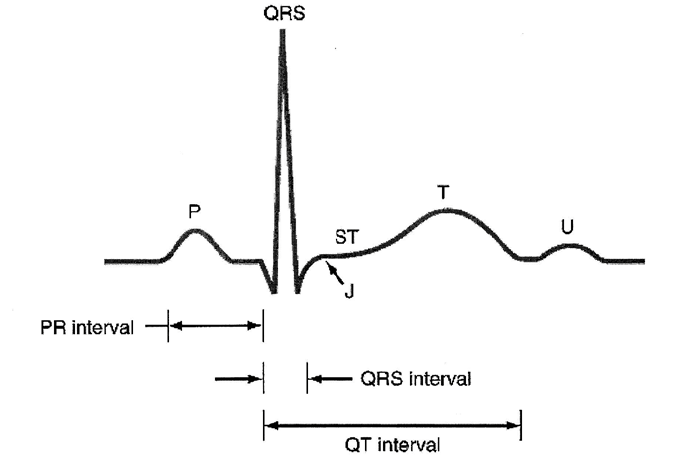
\includegraphics[width=0.6\textwidth]{./Exp1/pic/image5.png}
    \end{center}
    \caption{Sample Voltage Pattern for ECG}
    \label{fig:ecgpattern}
\end{figure}

The canonical example in medicine for measuring voltage potentials and displaying them (with an oscilloscope) are ECG (Electrocardiography) and EEG (Electroencephalography). The basic idea of these two standard devices is fairly simple: by measuring the potential difference in time between two points (or usually several pairs of points) one gets a nice direct insight into the activity of the heart (brain) and can therefore detect dysfunctions easily. Let us, for example, take a closer look at how an ECG works: If you record the electrical potential between two points along your chest you can record the voltage pattern shown in figure \ref{fig:ecgpattern} (in time).\footnote{Remember: The ECG only shows the electrical polarization of the heart muscle. It does not show the contraction of the heart muscle!} \myskip

As you can see, the pattern observed can be split into different parts: At first the atrial cells are depolarized, giving the first signal (P wave). (This signal is relatively weak due to the small mass of the atrium.) After a delay one gets the QRS complex, which indicates the depolarization (wave) of the ventricles. After another delay one gets the T wave, which comes from the repolarization of the heart. \footnote{The interpretation of the U wave is still not yet 100\% understood} What do all these results, obtained from the heart as a total, mean in terms of processes going on in the single cells? The next figure \ref{fig:ventricule} shows the measurement by your ECG in comparison to the potential in a single cell in a ventricle (obtained using a different method). First we recall that the interior and the exterior of the cell in their standard state have different ion concentrations and are therefore at different electrical potentials. (That is the zero line in the graph.) In the depolarization phase the ion channels in the cell membrane open and a flow of $\mathrm{K}^+$ ions changes the potential inside the cell very rapidly. After this rapid change in potential one gets a plateau, which is mainly due to the inflow of $\mathrm{Ca}^{++}$ ions into the cell. (The $\mathrm{Ca}^{++}$ ions are much bigger than the $\mathrm{K}^+$ ions, because they have a much larger hydrogen cover surrounding them and they diffuse much slower through the ion channels.) Finally in the repolarization phase the ion channels close again and the ion pumps in the cell membrane reestablish the initial ion concentrations. \myskip

\begin{figure}[h]
    \begin{center}
        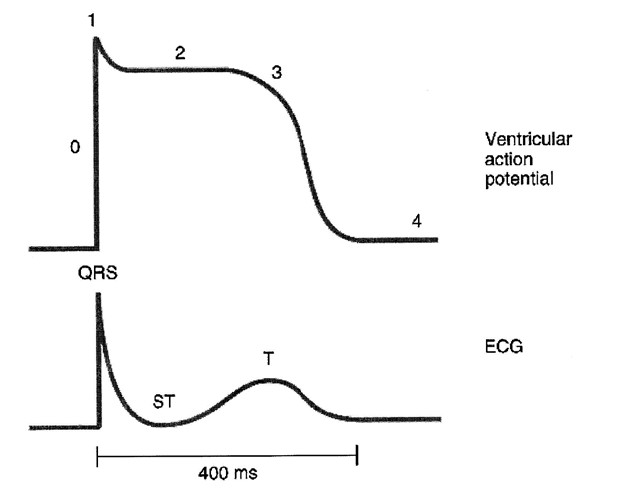
\includegraphics[width=0.55\textwidth]{./Exp1/pic/image6.png}
    \end{center}
    \caption{Comparison with Ventricular Potential}
    \label{fig:ventricule}
\end{figure}

How can you now take advantage of this method for a diagnosis? First of all you don't want to take the measurements only along one single axis or plane, since e.g.\ if an infarction occurs on the front or back wall of your heart you are probably going to miss it. These days the usual way to get a 3-D picture of the position of the heart axis\footnote{The heart axis is a simplified concept of the locations of the electrical potentials in the heart. One can think of the heart axis as a vector symbolizing the (physical) axis of the heart.} is obtained by measuring with multiple channels simultaneously between the points indicated in figure \ref{fig:channels}. (The contacts with an R are placed on the patients back.) \myskip

\begin{figure}[h]
    \begin{center}
        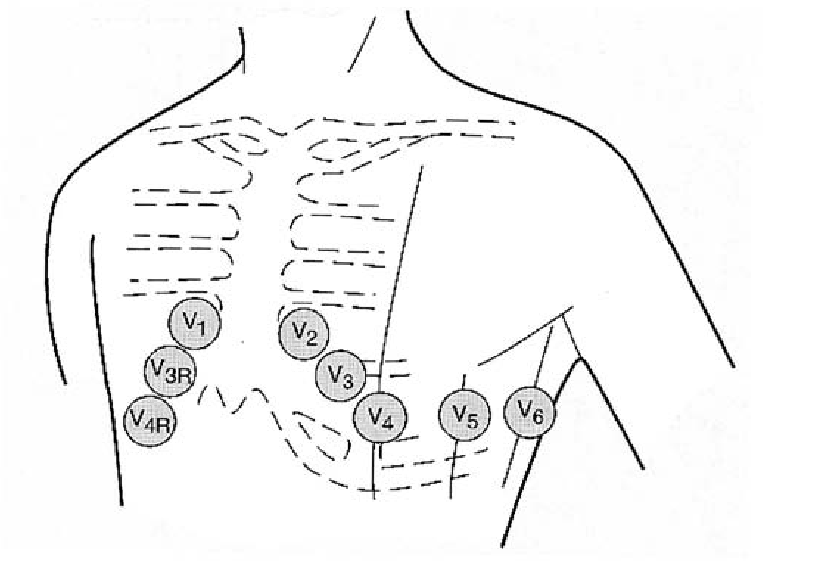
\includegraphics[width=0.5\textwidth]{./Exp1/pic/image7.png}
    \end{center}
    \caption{Channels of Measurement}
    \label{fig:channels}
\end{figure}

\begin{figure}[h]
    \begin{center}
        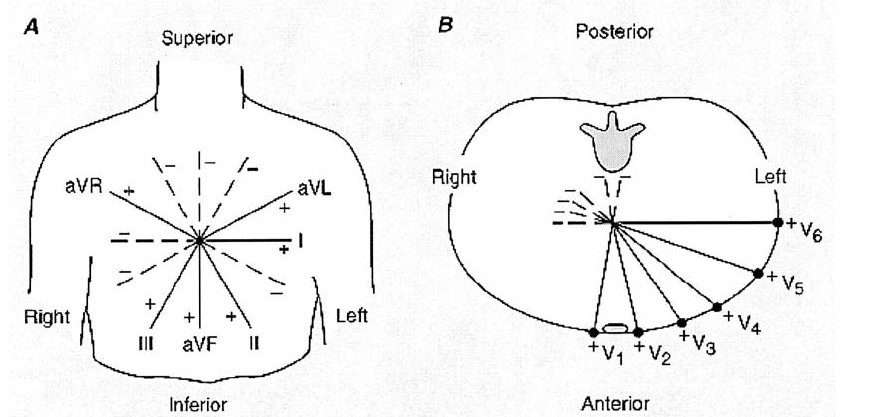
\includegraphics[width=0.8\textwidth]{./Exp1/pic/image8.png}
    \end{center}
    \caption{Electric Potentials and Information}
    \label{fig:heartcomp}
\end{figure}

From the location and amplitude of the main vector (axis) one can see for example if the muscle mass is increased on one side of the heart (hypertrophy). In that case the main vector is tilted.\footnote{Also in pregnant women the heart as a total is slightly repositioned and therefore the electrical axis is a little bit off.} Another thing to look for is if the depolarization and repolarization was performed properly. For example if the ion channels in a certain region of the heart are destroyed by an infarction, then the electric potential between the depolarization and repolarization phase does not reach the zero level. By looking at your data you can not only locate the infarction, but also read off additional information, e.g.\ if the infarction killed the tissue through all of the heart wall or only parts of it. (That determines your treatment of the patient!) \myskip

You can see that you can get a lot of useful information if you look at electrical potentials (and their change in time), as shown in figure \ref{fig:heartcomp}. \myskip

Textbook references:
\begin{enumerate}
    \item Stein: \emph{Internal Medicine}
    \item Harrison's \emph{Principles of Internal Medicine}
\end{enumerate}

\newpage
\section{Lab Preparation Examples}

\noindent\underline{Field Lines}: Given the following equipotential lines, draw 5-10 field lines on each diagram. \myskip

\begin{minipage}[h]{0.95\textwidth}
    1.\begin{center}
        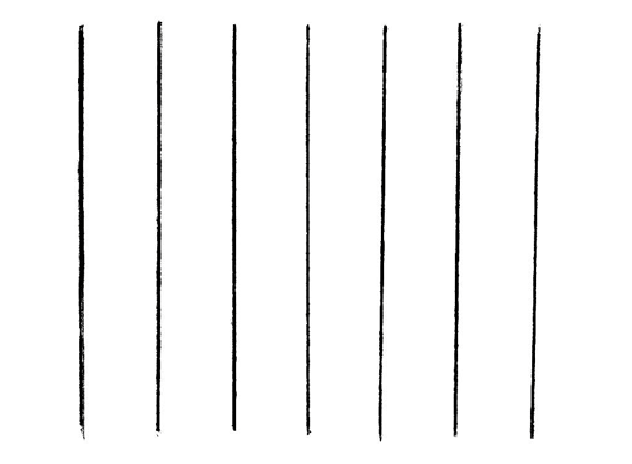
\includegraphics[width=0.7\textwidth]{./Exp1/pic/image9.png}
    \end{center}
\end{minipage}

\begin{minipage}[h]{0.95\textwidth}
    2.\begin{center}
        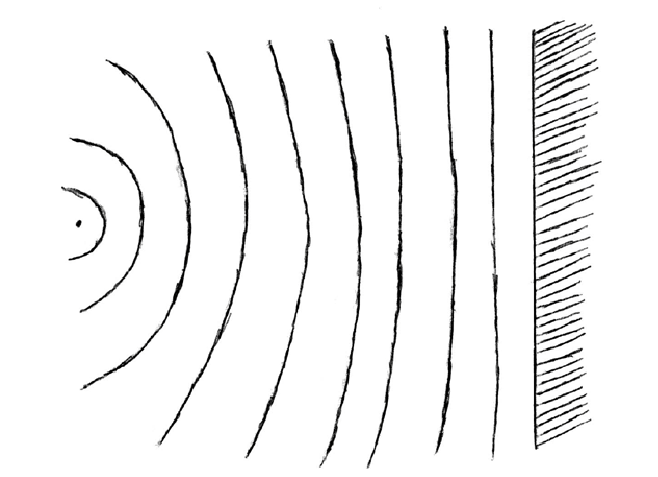
\includegraphics[width=0.7\textwidth]{./Exp1/pic/image10.png}
    \end{center}
\end{minipage}

\begin{minipage}[h]{0.95\textwidth}
    3.\begin{center}
        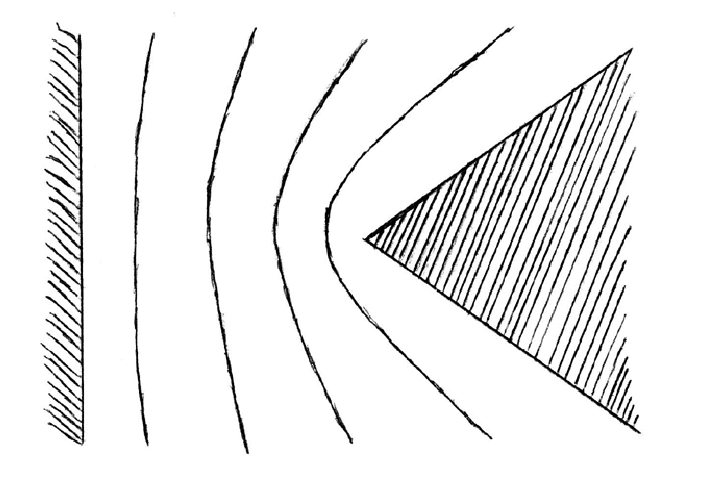
\includegraphics[width=0.7\textwidth]{./Exp1/pic/image11.png}
    \end{center}
\end{minipage}

\begin{minipage}[h]{0.95\textwidth}
    4.\begin{center}
        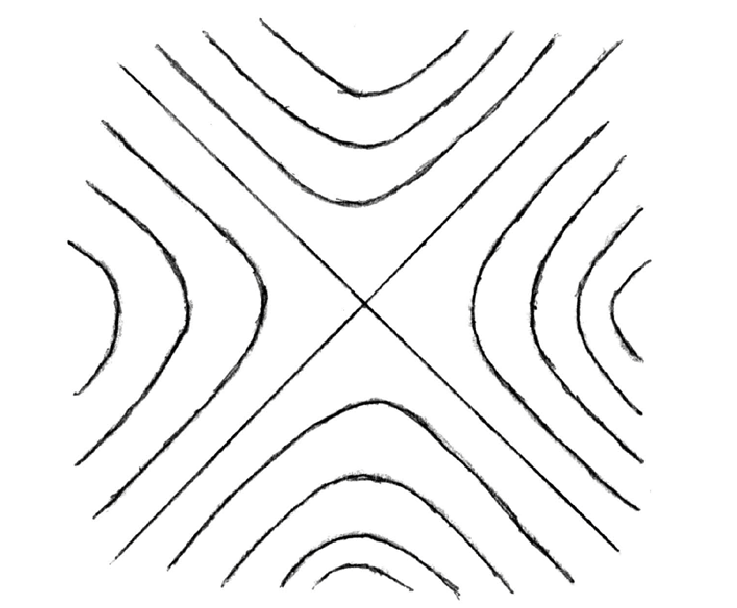
\includegraphics[width=0.7\textwidth]{./Exp1/pic/image12.png}
    \end{center}
\end{minipage}

\noindent\underline{Shield Theorem} \myskip

5. Explain in a few sentences why you might be safe inside your new Volkswagen Beetle even when struck by a bolt of lightning.
